\documentclass[journal]{IEEEtran}

\usepackage{aligned-overset}












\ifCLASSINFOpdf
 
\else

\fi





%

\hyphenation{op-tical net-works semi-conduc-tor}


\begin{document}



\title{Report for Reading Paper\\ A Generalized Path Integral Control Approach to Reinforcement Learning}





\author{Yunian Pan}




% make the title area
\maketitle

% As a general rule, do not put math, special symbols or citations
% in the abstract or keywords.
\begin{abstract}

This Report presents some substances of the paper "A Generalized Path Integral Control Approach to Reinforcement Learning", as the paper stated: "reinforcement learning has recently moved towards
combining classical techniques from optimal control and dynamic programming with modern learning techniques from statistical estimation theory in order to develop more scalable algorithms
with higher efficiency and fewer open parameters, the paper suggests to use the framework of stochastic optimal control with path integrals calle $PI^2$ to do parameterized policy approximation,  
 value function estimation and optimal control based on the stochastic Hamilton-Jacobi-Bellman (HJB) equations."
 
The algorithm's only parameter is the exploration noise, it can be conceived of as model-based, hybrid, or even model free,
depending on how the learning task is structured. 
The update equations have no danger of
numerical instabilities because neither matrix inversions nor gradient learning rates are required. 

This report will briefly present the theoretical development of the original paper, then show the experimental set up and results, some Discussion
required by the assignments will be given.



\end{abstract}
\ \\
% Note that keywords are not normally used for peerreview papers.
\begin{IEEEkeywords}
stochastic optimal control, reinforcement learning, parameterized policies, path integrals.
\end{IEEEkeywords}






% For peer review papers, you can put extra information on the cover
% page as needed:
% \ifCLASSOPTIONpeerreview
% \begin{center} \bfseries EDICS Category: 3-BBND \end{center}
% \fi
%
% For peerreview papers, this IEEEtran command inserts a page break and
% creates the second title. It will be ignored for other modes.
\IEEEpeerreviewmaketitle


\ \\
\section{Summary}

\subsection{Brief theoretical development}

The theoretical development can be divided into 4 parts, the first part is how we can start to derive stochastic optimal control algorithm from Hamiltan-Jacobian-Bellman equation(HJB),
the optimal control of a general stochastic control framework can be derived from following nonlinear PDE,
\begin{equation}
    \begin{aligned}
    -\partial_t V_t = q_t + (\nabla_xV_t)^{\top}f_t -\frac{1}{2}(\nabla_xV_t)^{\top}G_tRd^{-1}G_t^{\top}(\nabla_{x_t}V_t) \\
     + \frac{1}{2}trace((\nabla_{xx}V_t)G_t\Sigma_{\epsilon}G_t^{\top})
    \label{nonlinear PDE}
    \end{aligned}
  \end{equation}

The second part is to make a logarithmic transfrom of this nonlinear PDE so that we get a linear PDE, here we make a very some strong assumptions that:
\begin{equation}
  \lambda G_t R^{-1}G_t^{\top} = G_t \Sigma_{\epsilon}G_t^{\top} = \Sigma(x_t)
  \label{assumption1}
\end{equation}
This assumption implies that the cost of the control is \underline{inverse proportional to the noise variance}, and using Feyman-Kac lemma we can solve this PDE as a path integral:
\begin{equation}
    \Psi_{t_i} = \lim_{dt\to 0}\int p(\tau_i|x_{t_i}) \exp[-\frac{1}{\lambda}(\phi_{t_N}+\sum_{j=i}^{N-1}q_{t_j}dt)]d\tau_i
    \label{solution1}
  \end{equation}


The third part is to do some formulation of the MDP process and building the probability of the trajectory through Gaussian noise distribution,
since the only stochastic part is the noise, we would get an explicit expression of the trajectory cost, and through the expression we can derive the
optimal stochastic control which can be viewed as the probability combination of local optimal control.(This actually results in stochastic optimal control algorithm,
but people don't like it since it's too complicated!)

The forth part is to parametrize the policy, and start from a simple DMP case,(which will be discarded later to prove this algorithm can be model free) we get the parameter updating formula:
\begin{equation}
    \begin{aligned}
    \theta^{(new)} &= \frac{1}{N} \sum_{i = 0}^{N-1} \delta \theta_{t_i} + \frac{1}{N} \sum_{i = 0}^{N-1} \theta \\
    & = \frac{1}{N} \sum_{i = 0}^{N-1} \delta \theta_{t_i} + \theta
    \end{aligned}
   \end{equation}

  Thus the main framework of \textbf{P}olicy \textbf{I}mprovement with \textbf{P}ath \textbf{I}ntegrals (PI$^2$) has been constructed, with the equations below:

   \begin{equation}
     \begin{aligned}
       P(\tau_i) & = \frac{e^{-\frac{1}{\lambda}S(\tau_i)}  }{\int e^{-\frac{1}{\lambda}S(\tau_i)}d\tau_i} \nonumber  \\
      S (\tau_i)& = \phi_{t_N}+\sum_{j=i}^{N-1}q_{t_j} \\ & + \frac{1}{2}\sum_{j=i}^{N-1}  \frac{1}{2}(\theta_{t_j} + \epsilon_{t_j})^{\top}{R}^{-1} (\theta_{t_j} + \epsilon_{t_j})\\ 
      \delta \theta_{t_i} & = \int P(\tau_i) M_{t_i} \epsilon_{t_i} d\tau_i \\
      [\delta \theta ]_j &=  \frac{\sum_{ i= 0}^{N-1}(N-i)w_{j, t_i}[\delta \theta_{t_i}]_j}{\sum_{ i= 0}^{N-1}(N-i)w_{j, t_i}} \\ 
      \theta^{(new)} & = \theta^{(old)} + \delta \theta
     \end{aligned}
   \end{equation}
  
It's remarkable that in the derivation we actually discard another projection matrix term in order to get time invariant policy!


\subsection{How was it done?}

Analogous to the generalized formulation of stochastic optimal control with path integrals, the algorithm 
was derived using the constructed equations, 
$\ref{table 1}$ describes the algorithm.

\begin{table}
    \caption{}
    \label{table 1}
     \begin{itemize}
       \item[$\bullet$] Given: 
       \begin{itemize}
         
         \item The immediate cost: $r_t = r(x_t,u_t,t) = q_t + \frac{1}{2} \theta_t^{\top} R \theta_t$
         \ \\
         \item A terminal cost term $\Phi_{t_N}$
         \ \\
         \item A stochastic parameterized policy $\alpha_{t_i} = g_{t_i}^{\top} (\theta + \epsilon_{t_i})$
         \ \\
         \item The basis function $g_{t_i}$ from the system dynamics
         \ \\
         \item The variance $\Sigma_{\epsilon}$ of the mean zero noise $\epsilon_t$
         \ \\
         \item The initial parameter vector $\theta$ 
       \end{itemize}  
        \ \\
       \item[$\bullet$] Repeat until convergence of the tracjectory cost $S$
       \begin{itemize}
         
         \item Create K roll-outs of the system from the same start state $x_0$ using stochstic parameters
         $\theta+ \epsilon_t$ at every time step
         \ \\
         \item For $k = 1 , \ldots,  K$, compute:
         \ \\
         \begin{itemize}
          \item 
              $P(\tau_{i,k}) = \frac{e^{-\frac{1}{\lambda}S(\tau_{i,k})}}{\sum_{k=1}^{K} [e^{-\frac{1}{\lambda}S(\tau_{i,k})}]}  $
          \ \\
          \item $S(\tau_{i,k}) = \phi_{t_N,k}+\sum_{j=i}^{N-1}q_{t_j,k}   + \frac{1}{2}\sum_{j=i}^{N-1}  \frac{1}{2}(\theta + M_{t_j,k}\epsilon_{t_j,k})^{\top}{R}^{-1} (\theta + M_{t_j,k}\epsilon_{t_j,k})$
          \ \\
          \item $M_{t_j, k} = \frac{R^{-1}g_{t_j, k}g_{t_j, k}^{\top}}{g_{t_j, k}^{\top}R^{-1}g_{t_j, k}}$
         \end{itemize}
         \ \\
         \item Probability of a trajectory: $P(\tau_i) = \frac{e^{-\frac{1}{\lambda}\tilde{S}(\tau_i)}  }{\int e^{-\frac{1}{\lambda}\tilde{S}(\tau_i)}d\tau_i}$ 
         \ \\
         \item Generalized trajectory cost: $\tilde{S}(\tau_i) = S(\tau_i) + \frac{\lambda}{2} \sum_{j = i}^{N-1} \log |H_{t_j}|$
          \ \\
         \item Local controls: $u_L(\tau_i) = R^{-1} {G_{t_i}^{(c)}}^{\top} ({G_{t_i}^{(c)}} R^{-1} {G_{t_i}^{(c)}}^{\top})^{-1}(G_{t_i}^{(c)}\epsilon_{t_i} - b_{t_i})$
       \end{itemize} 
       \ \\
       \item For $i=1, \ldots, (N-1)$,compute:
       \ \\ 
       \begin{itemize}
        \item  $\delta \theta_{t_i}  = \sum_{k=0}^{K}[ P(\tau_{i,k}) M_{t_{i,k}} \epsilon_{t_{i,k}}  ]$
        \ \\ 
       \end{itemize}
       \item Compute: $[\delta \theta ]_j =  \frac{\sum_{ i= 0}^{N-1}(N-i)w_{j, t_i}[\delta \theta_{t_i}]_j}{\sum_{ i= 0}^{N-1}(N-i)w_{j, t_i}}$
       \ \\
       \item Update: $ \theta^{(new)}  = \theta^{(old)} + \delta \theta$
       \ \\
       \item Create one noiseless roll-out to check the trajectory cost $R = \Phi_{t_N} +\sum_{i = 0}^{N -1} r_{t_i}$ . In case
       the noise cannot be turned off, that is, a stochastic system, multiple roll-outs need be averaged.
     \end{itemize}
   
   \end{table}


\subsection{Why is it worth doing?}

Cited from the original paper: It's simple formed, numerically robust in high dimensional problems, with no open algorithmic tuning parameters except exploration noise. What's more, it makes interesting connection to previous work on RL based on
probability matching and motivates why probability matching algorithms can be successful. In general,
Policy Improvement with Path Integrals ($\mbox{PI}^2$) offers currently one of the most efficient, numerically robust, and easy to implement algorithms for RL based on trajectory roll-outs.


\subsection{results}
There were 3 learning tasks done in the paper:
\subsubsection{ 1 DOF Via-Point Task}

Forcing the movement to pass through an intermediate via-point at a particular time, which is an abstract approximation of hitting a
target.
The cost function was:

\begin{equation} 
  \begin{aligned}
    r_{300ms} &= 100000000(G- y_{t_{300ms}})^2 \\
    \phi_{t_N} &= 0  \nonumber 
  \end{aligned}
\end{equation}

with $G = 0.25$. 
The results shown in $\ref{1dofv}$ indicates that PI$^2$ performs the best:
\begin{figure}[htbp]
  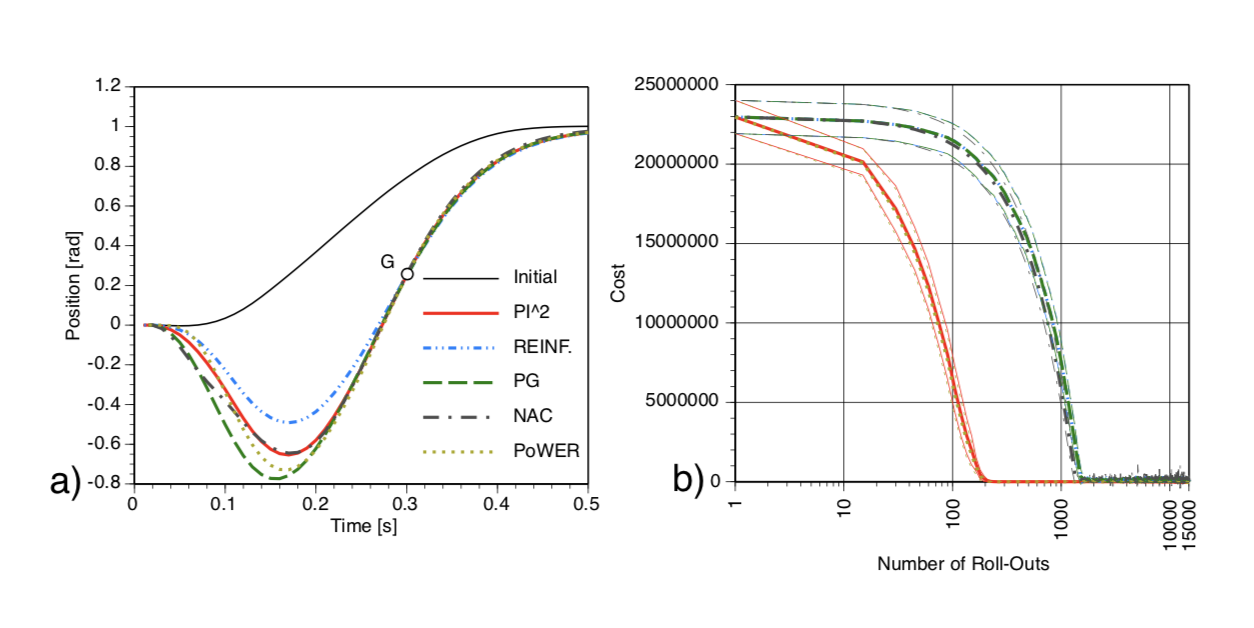
\includegraphics[width = .5\textwidth]{1dofv}
  \caption{1 DOF via-point comparison}
  \label{1dofv}
\end{figure}

\subsubsection{Multi-DOF Via-Point Task}

The learning task was to pass through an intermediate target, just that a d = 2, 10, 50 dimensional motor primitive was employed thus result in a redundant learning 
problem. 
Denote the joint angles of the robots as $\xi_i,\ i=1,\ldots,d $, s.t. the directly actuated part is: 
$\ddot{\xi_{i,t}} = f_{i, t} + g_{i, t}^{\top}(\theta_i + \epsilon_{i,t})$, The end-effector position is computed as: 

\begin{equation}
  \begin{aligned}
    x_t = \frac{1}{d} \sum_{i=1}^{d}\cos(\sum_{j=1}^{i}\xi_{j,t}) \\
    y_t = \frac{1}{d} \sum_{i=1}^{d}\sin(\sum_{j=1}^{i}\xi_{j,t}) \nonumber 
  \end{aligned}
\end{equation}

The cost function was designed as:

\begin{equation} 
  \begin{aligned}
    r_t &= \frac{\sum_{i=1}^{d}(d+1-i)(0.1f_{i,t}^2+ 0.5\theta_i^{\top}\theta_i)}{\sum_{i=1}^{d}(d+1-i)} \\
    \Delta r_{300ms} &= 10^8((0.5 - x_{t_{300ms}})^2+(0.5 - y_{t_{300ms}})^{2})  \nonumber \\ 
    \phi_{t_N} &= 0 
  \end{aligned}
\end{equation}

The comparison shown in $\ref{mdofv}$ indicates that PI$^2$ is superior to others.

\begin{figure}[htbp]
  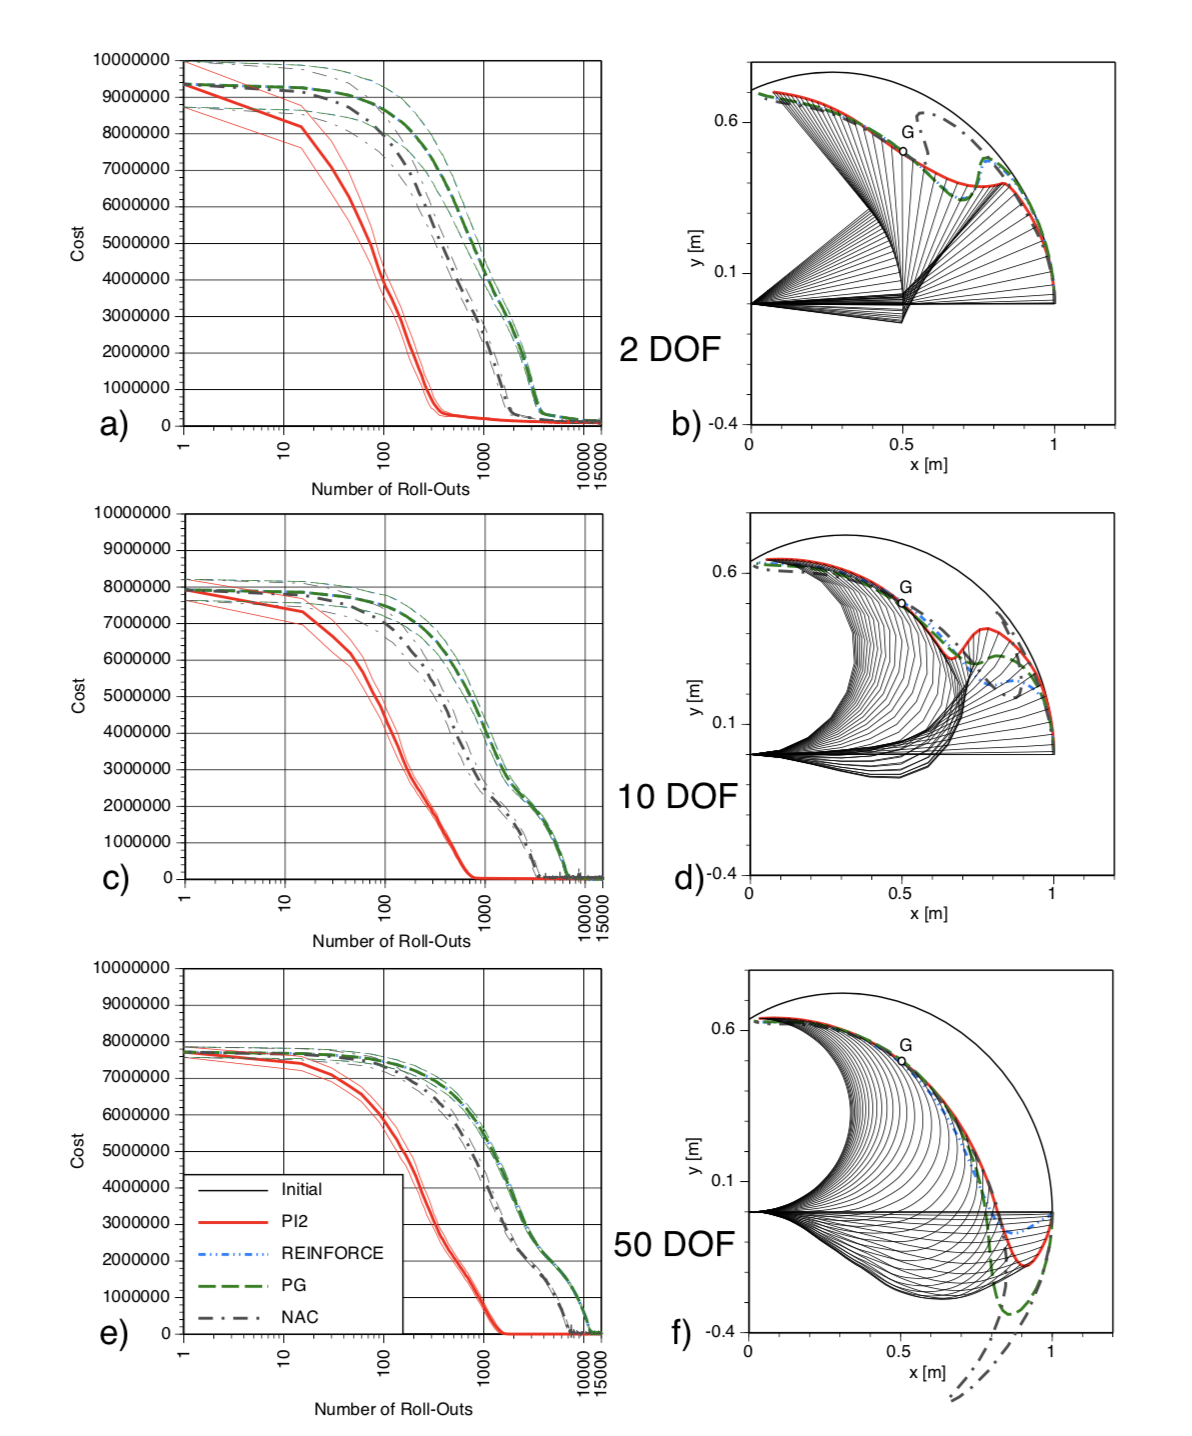
\includegraphics[width = .5\textwidth]{mdofv}
  \caption{multi-DOF via-point comparison}
  \label{mdofv}
\end{figure}

\subsubsection{Dog jumping}

The robot dog is to jump across as gap. The paper only uses a simulation to show the results as real robot was not available. 
The dog has 3 DOFs per leg, thus a total of d=12, each DOF represented with 50 basis functions. 

PI$^2$ learning used primarily the forward progress as a reward, a penalty was incurred if the yaw or the roll exceeded a threshold value, which encouraged the
robot to jump straight across the gap instead of to the side or falling over. The exact cost design is:

\begin{equation} 
  \begin{aligned}
    r_t &= r_{roll}+ r_{yaw} + \sum_{i=1}^{d}(a_1 f_{i,t}^2 + 0.5a_2 \theta_i^{\top}\theta_i) \\
  r_{roll} &= \left\{ \begin{array}{rcl} &100(|roll_t|-0.3)^2 & if |roll_t|>3 \\ &0 &otherwise \end{array} \right. \nonumber \\ 
  r_{yaw} &= \left\{ \begin{array}{rcl} &100(|yaw_t|-0.1)^2 & if |yaw_t|>0.1 \\ &0 &otherwise \end{array} \right. \nonumber \\
    \phi_{t_N}& = 5 \times 10^{4} (goal -x_{nose})^2,   
  \end{aligned}
\end{equation}

Roll and yaw are the roll and yaw angles of the robot's body, and $x_{nose}$ is the position of the "nose".
The multipliers for each reward component were tuned to have a balanced influence of all terms. Ten learning trials were performed initially for the first parameter update.
 
\begin{figure}[htbp]
  \centering
  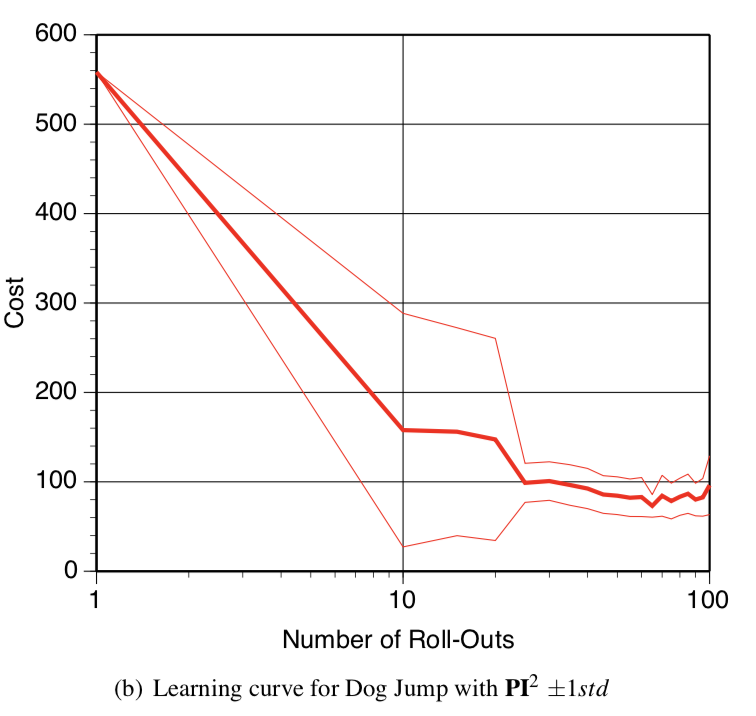
\includegraphics[width = .3\textwidth]{dog}
  \caption{learning curve}
  \label{dog}
\end{figure}

It should be noted that here manual tuning is focused on generating a good cost function, which is beyond the scope of reinforcement learning. 



\section{How the paper relates the algorithms seen in class?}

This algorithm has been presented in our class, as we are entering the era of DQN, we learned that we can use a parametrized function to
approximate the best policy, in the context of this idea and after some beautiful mathematical development and derivations, Theodorou et. came
up with this idea which can be model-based semi-model based and even model-free, thus give the readers infinite possibility to solve many 
reinforcement learning tasks. What's more, the algorithm, absorbing some nice property of Monte-Carlo sampling, provides a
 very mathematically solid ground.



\section{Discussion}

As can be seen from the previous figures, the PI$^2$ Algorithm has a surprisingly good performance, without any need for tuning parameters. And it's scalable to high dimensionality.
Yet there's indeed space to improve such as the cost function design, which future work might be focus on to move the algorithm to a "black box" character.

The real beauty in the development is that through making a simple assumption but gigantically reduce the complexity of the PDE equation, future work might also fall into the effort
of removing this assumption or change it into more generalized version.
% if have a single appendix:
%\appendix[Proof of the Zonklar Equations]
% or
%\appendix  % for no appendix headi
% do not use \section anymore after \appendix, only \section*
% is possibly needed

% use appendices with more than one appendix
% then use \section to start each appendix
% you must declare a \section before using any
% \subsection or using \label (\appendices by itself
% starts a section numbered zero.)
%




% you can choose not to have a title for an appendix
% if you want by leaving the argument blank



% use section* for acknowledgment



% Can use something like this to put references on a page
% by themselves when using endfloat and the captionsoff option.
\ifCLASSOPTIONcaptionsoff
  \newpage
\fi



% trigger a \newpage just before the given reference
% number - used to balance the columns on the last page
% adjust value as needed - may need to be readjusted if
% the document is modified later
%\IEEEtriggeratref{8}
% The "triggered" command can be changed if desired:
%\IEEEtriggercmd{\enlargethispage{-5in}}

% references section

% can use a bibliography generated by BibTeX as a .bbl file
% BibTeX documentation can be easily obtained at:
% http://mirror.ctan.org/biblio/bibtex/contrib/doc/
% The IEEEtran BibTeX style support page is at:
% http://www.michaelshell.org/tex/ieeetran/bibtex/
%\bibliographystyle{IEEEtran}
% argument is your BibTeX string definitions and bibliography database(s)
%\bibliography{IEEEabrv,../bib/paper}
%
% <OR> manually copy in the resultant .bbl file
% set second argument of \begin to the number of references
% (used to reserve space for the reference number labels box)
\begin{thebibliography}{1}

\bibitem{Theodo}Theodorou, Evangelos, Jonas Buchli, and Stefan Schaal. "A generalized path integral control approach to reinforcement learning." journal of machine learning research 11.Nov (2010): 3137-3181.

\end{thebibliography}





\end{document}
